\chapter{Generaliseringer af lasso estimatoren} \label{ch:generalisering_lasso}
\textit{I dette kapitel beskrives nogle generaliseringer af standard lasso herunder elastisk net, group lasso og adaptive lasso.
Disse procedurer har alle de to essentielle egenskaber af standard lasso: shrinkage og udvælgelse af variable eller grupper af variable.}

\section{Elastisk net}
I dette afsnit introduceres en shrinkage metode kaldet elastisk net, som kombinerer ridge regression og lasso.
Metoden blev først præsenteret i \citep{zou_hastie}.

Selvom lasso har vist succes i mange tilfælde, har den også nogle begrænsninger:
%
\begin{enumerate}[label=\textnormal{(\arabic*)}]
    \item Hvis $p>n$, da udvælger lasso højst $n$ variable, hvilket kommer af, at lasso er et konvekst optimeringsproblem. Derudover er lasso ikke veldefineret medmindre \(\Vert \beta \Vert_1 \leq t\). \label{itm:1}
    \item Hvis der eksisterer en gruppe af variable, som har høj parvis korrelation, da har lasso en tendens til blot at udvælge  én variabel fra denne gruppe og denne variabel udvælges tilfældigt. \label{itm:2}
    \item Hvis $n>p$ og der er høj korrelation mellem variablerne, da er det empirisk bevist at prædiktions performance af lasso er domineret af ridge regression \citep{lasso}.  \label{itm:3}
\end{enumerate}
%
Målet er at finde en metode, som overkommer ovenstående begrænsninger.
%
\begin{defn}[Naiv elastisk net]
Antag responsvariablen er centreret og prædiktorerne er standardiseret, da er det naive elastiske net givet ved
\begin{align}
\hat{\tbeta}^\text{naivEN} = \argmin_{\tbeta} \cbr{\Vert \y - \X \tbeta \Vert_2^2 + \lambda_2 \Vert \tbeta \Vert_2^2 + \lambda_1 \Vert \tbeta \Vert_1}, \label{eq:naivEN}
\end{align}
for \(\lambda_1, \lambda_2 \geq 0\).
\end{defn}
%
Lad \(\alpha = \frac{\lambda_1}{\lambda_1 + \lambda_2}?????\), da er \eqref{eq:naivEN} ækvivalent med optimeringsproblemet
\begin{align*}
\hat{\tbeta}^\text{naivEN} = \argmin_{\tbeta} \cbr{\Vert \y - \X \tbeta \Vert_2^2}, \ \text{underlagt at } \frac{1}{2}\del{1-\alpha} \Vert \tbeta \Vert_2^2 + \alpha \Vert \tbeta \Vert_1 \leq t,
\end{align*}
som kan omskrives til et Lagrange problem
\begin{align}
\hat{\tbeta}^\text{naivEN} =\argmin_{\tbeta} \cbr{ \Vert \y - \X \tbeta \Vert_2^2 + \lambda \sbr{\frac{1}{2}(1- \alpha) \Vert \tbeta \Vert_2^2 + \alpha \Vert \tbeta \Vert_1}}. \label{eq:4.2}
\end{align}
Hvis $\alpha=0$, da reduceres det til den kvadrerede $\ell_2$-norm svarende til strafleddet for ridge regression og hvis $\alpha=1$ reduceres strafleddet til $\ell_1$-normen svarende til strafleddet for lasso.
Optimeringsproblemet  \eqref{eq:4.2} er streng konveks for \(\alpha \in [0,1)\), hvilket betyder, at der eksisterer en entydig løsning uafhængigt af korrelationsstrukturen af $\X$.
For  \(\alpha=1\) er problemet konveks, men ikke streng konveks.
Dette ses tydeligt på figur \ref{fig:elastisk}.
%
\begin{figure}[H]
\centering
\scalebox{0.8}{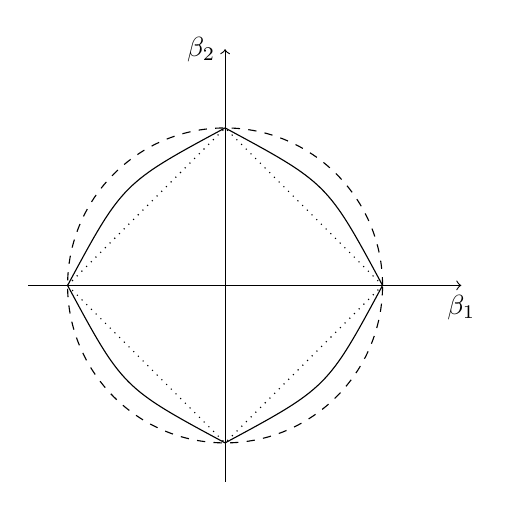
\begin{tikzpicture}
\draw[dashed] (0,0) circle (2cm);
\draw[dotted] (-2,0) -- (0,-2) -- (2,0) -- (0,2) -- (-2,0); 
\draw (-2,0) .. controls (-1.3,1.3) .. (0,2);
\draw (0,2) .. controls (1.3,1.3) .. (2,0);
\draw (-2,0) .. controls (-1.3,-1.3) .. (0,-2);
\draw (0,-2) .. controls (1.3,-1.3) .. (2,0);
\draw [<-] (0,3) node [left] {$\beta_2$}-- (0,-2.5);
\draw[<-] (3,0) node [below] {$\beta_1$} -- (-2.5,0);
\end{tikzpicture}}
\caption[optional short text]{To dimensional illustration af betingelsesområderne for shrinkage metoderne: ridge regression (\tikz[baseline]{\draw[dashed] (0,.5ex)--++(.5,0) ;}), lasso (\tikz[baseline]{\draw[dotted] (0,.5ex)--++(.5,0) ;}) og elastisk net med \(\alpha = 0.5\) (\tikz[baseline]{\draw (0,.5ex)--++(.5,0) ;}). Vi observerer, at singulariteter i hjørnerne og kanterne er streng konveks. Styrken af konveksitet varierer med \(\alpha\).} \label{fig:elastisk}
\end{figure}
%
%\imgfigh{crime_el_lasso.pdf}{0.7}{Koefficientstierne for henholdsvis lasso og elastisk net med \(\alpha=0.3\) plottet imod log af $\lambda$ for crime data.}{crime_el_lasso}
%
%\begin{figure}[H]
%\centering
%\begin{minipage}{0.4\linewidth}
%\scalebox{0.32}{\includegraphics{fig/img/crime_lasso.png}}
%\end{minipage}
%\hspace{0.2cm}
%\begin{minipage}{0.4\linewidth}
%\scalebox{0.32}{\includegraphics{fig/crime_EN.png}}
%\end{minipage}
%\caption{Koefficientstierne for henholdsvis lasso (ventre) og elastisk net med \(\alpha=0.3\) (højre) plottet imod \(\ell_1\)-normen for crime data.} \label{fig:crime_koef_EN}
%\end{figure}
%
%En tre dimensionel illustration af betingelsesområderne for det elastiske net og standard lasso er givet på figur \ref{fig:elastisk_net}.
%Heraf ses at det elastiske net har egenskaberne af både $\ell_1$ kuglen og $\ell_2$ kuglen: de skarpe hjørner og kanter opfordrer til variable udvælgelse, mens de kurvede konturer opfordrer stærk korreleret variable til at dele koefficienter.
%%
%\begin{figure}[H]
%\centering
% \scalebox{0.5}{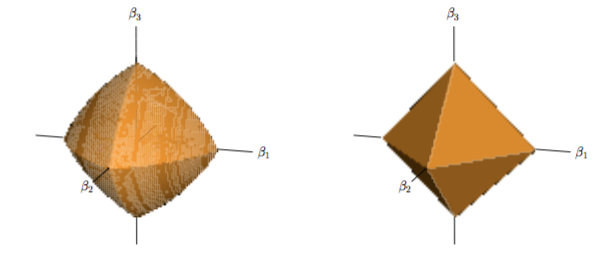
\includegraphics{fig/elastisk_net.jpg}}
%\caption{Kuglen for elastisk net med \(\alpha=0.7\) (venstre) og \(\ell_1\) kuglen (højre) i tre dimensioner.}
%\label{fig:elastisk_net}
%\end{figure}
%
Det viser sig, at optimeringsproblemet for naiv elastisk net kan transformeres til et ækvivalent lasso problem på augmented data.
%
\begin{lem} \label{lem:elastisk_net}
Givet data \(\del{\y, \X}\) og parametrene \(\del{\lambda_1, \lambda_2}\), defineres et augmented datasæt 
\begin{align*}
\X^* = \del{1 + \lambda_2}^{-1/2} \begin{pmatrix}
\X \\ \sqrt{\lambda_2} \mathbf{I}_p
\end{pmatrix}, \quad \y^* = \begin{pmatrix}
\y \\ \mathbf{0}
\end{pmatrix},
\end{align*}
hvor \(\X^* \in \mathbb{R}^{\del{n+p} \times p}\) og \(\y^* \in \mathbb{R}^{n+p}\).
Lad \(\gamma = \frac{\lambda_1}{\sqrt{1+\lambda_2}}\) og \(\tbeta^* = \sqrt{1+\lambda_2} \tbeta^\text{naivEN}\), da kan \eqref{eq:naivEN} omskrives til
\begin{align}
\hat{\tbeta}^* = \argmin_{\tbeta^*} \cbr{ \Vert \y^* - \X^* \tbeta^* \Vert_2^2 +\gamma \Vert \tbeta^* \Vert_1}, \label{eq:EN11}
\end{align}
hvor
\begin{align*}
\hat{\tbeta}^\text{naivEN} = \frac{1}{\sqrt{1+\lambda_2}} \hat{\tbeta}^*.
\end{align*}
\end{lem}
%
\begin{proof}
Vi har, at
\begin{align*}
\hat{\tbeta}^\text{naivEN} = \frac{1}{\sqrt{1+\lambda_2}} \hat{\tbeta}^*,
\end{align*}
hvor \(\hat{\tbeta}^*\) er givet i \eqref{eq:EN11}, således får vi, at
\begin{align*}
\hat{\tbeta}^\text{naivEN} &= \argmin_{\tbeta} \cbr{ \left\Vert \begin{pmatrix}
\y \\ \mathbf{0}
\end{pmatrix} -  \del{1 + \lambda_2}^{-1/2} \begin{pmatrix}
\X \\ \sqrt{\lambda_2} \mathbf{I}_p
\end{pmatrix} \sqrt{1+\lambda_2} \tbeta \right\Vert_2^2 + \frac{\lambda_1}{\sqrt{1+\lambda_2}} \left\Vert \sqrt{1+\lambda_2} \tbeta \right\Vert_1} \\
&= \argmin_{\tbeta} \cbr{ \left\Vert \begin{pmatrix}
\y \\ \mathbf{0}
\end{pmatrix} -  \begin{pmatrix}
\X \\ \sqrt{\lambda_2} \mathbf{I}_p
\end{pmatrix} \tbeta \right\Vert_2^2 + \lambda_1 \left\Vert \tbeta \right\Vert_1} \\
&= \argmin_{\tbeta} \cbr{ \left\Vert \begin{pmatrix}
\y - \X \tbeta \\ - \sqrt{\lambda_2} \tbeta 
\end{pmatrix} \right\Vert_2^2 + \lambda_1 \left\Vert \tbeta \right\Vert_1} \\
 &= \argmin_{\tbeta} \cbr{ \Vert \y - \X \tbeta \Vert_2^2 + \lambda_2 \Vert \tbeta \Vert_2^2 + \lambda_1 \Vert \tbeta \Vert_1}.
\end{align*}
\end{proof}
%Beviset følger af simpel algebra og er derfor undladt.
Da \(\X^*\) har rang \(p\), kan metoden i princippet altid vælge alle \(p\) prædiktorer.
Dermed er naiv elastisk net ikke begrænset til blot at vælge \(n\) prædiktorer hvis \(p > n\), som er tilfældet for lasso som beskrevet i punkt \ref{itm:1}.
Lemma \ref{lem:elastisk_net} viser også, at naiv  elastisk net udfører variabeludvælgelse svarende til lasso.
%
\begin{lem}
Hvis \(\X\) er ortogonal, da gælder, at
\begin{align}
\hat{\beta}_j^\text{ridge} &= \frac{\hat{\beta}_j^\text{OLS}}{1+\lambda_2}, \label{eq:orto_ridge} \\
\hat{\beta}_j^\text{lasso} &= \text{sign} \del{\hat{\beta}_j^\text{OLS}} \del{\left\vert \hat{\beta}_j^\text{OLS} \right\vert - \frac{\lambda_1}{2}}_+ =S_{\frac{\lambda_1}{2}} \del{ \hat{\beta}_j^\text{OLS}}, \label{eq:orto_lasso} \\
\hat{\beta}_j^\text{naivEN} &= \text{sign} \del{\hat{\beta}_j^\text{OLS}} \frac{\del{\left\vert \hat{\beta}_j^\text{OLS} \right\vert - \frac{\lambda_1}{2}}_+}{1+\lambda_2} = \frac{S_{\frac{\lambda_1}{2}} \del{ \hat{\beta}_j^\text{OLS}} }{1+\lambda_2} . \label{eq:orto_naivEN}
\end{align}
Figur \ref{fig:elastisk2} viser de operationelle egenskaber af ridge regression, lasso og naiv elastisk net, hvis \(\X\) er ortogonal. Heraf ses det også at naiv elastisk net er en two-stage procedure, først har vi en ridge lignende shrinkage, som efterfølges af en lasso lignende thresholding.
%
\begin{figure}[H]
\centering
\scalebox{0.8}{\begin{tikzpicture}
\draw[loosely dotted] (-3,-3) -- (3,3);
\draw[dotted] (-3,-2) -- (3,2);
\draw (-3,-1.5) -- (-0.75,0) -- (0.75,0) -- (3,1.5);
\draw[dashed] (-3,-2.2) -- (-0.75,0) -- (0.75,0) -- (3,2.2); 
\draw [<-] (0,3.5) node [left] {$\widehat{\beta}$}-- (0,-3.5);
\draw[<-] (3.5,0) node [below] {$\beta$} -- (-3.5,0);
\end{tikzpicture}
}
\caption[optional short text]{Eksakte løsninger for ridge regression (\tikz[baseline]{\draw[dotted] (0,.5ex)--++(.5,0) ;}), lasso (\tikz[baseline]{\draw[dashed] (0,.5ex)--++(.5,0) ;}) og naiv elastisk net (\tikz[baseline]{\draw (0,.5ex)--++(.5,0) ;}), hvis \(\X\) er ortogonal (\tikz[baseline]{\draw[loosely dotted] (0,.5ex)--++(.5,0) ;} OLS) for parametrene \(\lambda_1=2\) og \(\lambda_2=1\).} \label{fig:elastisk2}
\end{figure}
%
\end{lem}
%
\begin{proof}
Ridge estimatoren i det ortogonale tilfælde \eqref{eq:orto_ridge} følger direkte udfra ridge estimatoren \eqref{eq:ridge_estimator}, da \(\X^T \X = \mathbf{I}_p\) og \(\hat{\tbeta}^\text{OLS} = \X^T \y\).
For at bevise lasso estimatoren i det ortogonale tilfælde \eqref{eq:orto_lasso}, omskrives lasso problemet \eqref{eq:2.5} til følgende
\begin{align*}
\hat{\tbeta}^\text{lasso} &= \argmin_{\tbeta} \cbr{\del{\y - \X \tbeta}^T \del{\y - \X \tbeta} + \lambda_1 \Vert \tbeta \Vert_1} \\
&= \argmin_{\tbeta} \cbr{ \y^T \y - 2 \tbeta^T \X^T \y + \tbeta^T \X^T \X \tbeta + \lambda_1 \Vert \tbeta \Vert_1} \\
&= \argmin_{\tbeta} \cbr{- 2 \tbeta^T \hat{\tbeta}^\text{OLS} + \tbeta^T \tbeta + \lambda_1 \Vert \tbeta \Vert_1}.
\end{align*}
Lad os blot betragte indeks \(j\) af lasso estimatoren
\begin{align*}
\hat{\beta}_j^\text{lasso} = \argmin_{\beta_j} \cbr{ - 2 \beta_j \hat{\beta}_j^\text{OLS} + \beta_j^2 + \lambda_1 \vert \beta_j \vert}.
\end{align*}
Vi differentierer
\begin{align*}
\frac{\partial}{\partial \beta_j} \del{- 2 \beta_j \hat{\beta}_j^\text{OLS} + \beta_j^2 + \lambda_1 \vert \beta_j \vert}
=-2\hat{\beta}^\text{OLS} + 2\beta_j + \begin{cases}
-\lambda_1 \quad &\beta_j < 0 \\
[-\lambda_1, \lambda_1] & \beta_j = 0 \\
\lambda_1 & \beta_j >0 
\end{cases},
\end{align*}
dette sættes lig \(0\) og isolerer for \(\hat{\beta}_j\)
\begin{align*}
\hat{\beta}_j^\text{lasso} &= \hat{\beta}_j^\text{OLS} - \frac{1}{2}\begin{cases}
-\lambda_1 \quad &\beta_j < 0 \\
[-\lambda_1, \lambda_1] & \beta_j = 0 \\
\lambda_1 & \beta_j >0 
\end{cases} \\
&= \begin{cases}
\hat{\beta}_j^\text{OLS} + \frac{\lambda_1,}{2} \quad &\hat{\beta}_j^\text{OLS} < - \frac{\lambda_1}{2} \\
0, &\left\vert\hat{\beta}_j^\text{OLS} \right\vert \leq \frac{\lambda_1}{2} \\
\hat{\beta}_j^\text{OLS} - \frac{\lambda_1}{2}, \quad &\hat{\beta}_j^\text{OLS} > \frac{\lambda_1}{2}
\end{cases}. 
\end{align*}
Hvoraf vi får, at \(\hat{\beta}_j^\text{lasso} = S_{\frac{\lambda_1}{2}} \del{ \hat{\beta}_j^\text{OLS}} \), som fuldfører beviset.
Afslutningsvis følger naiv elastisk net estimatoren i det ortogonale tilfælde \eqref{eq:orto_naivEN} af \eqref{eq:orto_ridge} og \eqref{eq:orto_lasso}, da denne er en kombination heraf.
\end{proof}
%
Hvis vi har en gruppe af højt korreleret variable, da vil lasso blot udvælge én variabel og den udvælges tilfældigt, som nævnt i punkt \ref{itm:2}.
Men naiv elastisk net udvælger alle variable i denne gruppe, som vi nu vil vise. 
En regression metode udviser denne evne, hvis regressions koeffcienterne af en gruppe af højt korreleret variable er approksimativt ens.
%
\begin{lem} \label{lem:elastisk_net2}
Lad os betragte
\begin{align}
\hat{\tbeta} = \argmin_{\tbeta} \Vert \y - \X \tbeta \Vert_2^2 + \lambda J \del{\tbeta}, \label{eq:EN10}
\end{align}
hvor \(J \del{\cdot}\) er positiv for \(\tbeta \neq 0\).
Antag \(\x_i = \x_j\), for \(i, j = 1, \ldots, p\).
\begin{enumerate}[label=\alph*)]
\item Hvis \(J \del{\cdot}\) er streng konveks, da er \(\hat{\beta}_i = \hat{\beta}_j\), for alle \(\lambda \geq 0\).
\item Hvis \(J \del{\tbeta} = \Vert \tbeta \Vert_1\), da er \(\hat{\beta}_i \hat{\beta}_j \geq 0\) og \(\hat{\tbeta}^*\) er optimum af \eqref{eq:EN10}, hvor
\begin{align*}
\hat{\beta}_k^* = \begin{cases}
\hat{\beta}_k & k \neq i \text{ og } k \neq j, \\
\del{\hat{\beta}_i + \hat{\beta}_j} s & k = i, \\
\del{\hat{\beta}_i + \hat{\beta}_j} \del{1-s} & k = j,
\end{cases}
\end{align*}
for ethvert \(s \in \sbr{0,1}\).
\end{enumerate}
\end{lem}
%
\begin{proof}
Først bevises a).
Fasthold \(\lambda > 0\).
Hvis \(\hat{\beta}_i \neq \hat{\beta}_j\), lad os betragte \(\hat{\tbeta}^*\) som
\begin{align*}
\hat{\beta}_k^* = \begin{cases}
\hat{\beta}_k & k \neq i \text{ og } k \neq j, \\
\frac{1}{2} \del{\hat{\beta}_i + \hat{\beta}_j} & k = i \text{ eller } k = j.
\end{cases}
\end{align*}
Da \(\x_i = \x_j\), må vi have at \(\X \hat{\tbeta}^* = \X \hat{\tbeta}\) og dermed \(\Vert \y - \X \hat{\tbeta}^* \Vert_2^2 = \Vert \y - \X \hat{\tbeta} \Vert_2^2\).
Men da \(J \del{\cdot}\) er streng konveks, må vi have, at \(J \del{\hat{\tbeta}^*} < J \del{\hat{\tbeta}}\).
Dermed kan \(\hat{\tbeta}\) ikke være optimum af \eqref{eq:EN10}, som er en modstrid.
Derfor må vi have at \(\hat{\beta}_i = \hat{\beta}_j\).

Herefter bevises b).
Hvis \(\hat{\beta}_i \hat{\beta}_j < 0\), lad os igen betragte \(\hat{\tbeta}^*\) som ovenfor.
Da ser vi, at \(\vert \hat{\tbeta}^* \vert < \vert \hat{\tbeta} \vert\), så \(\hat{\tbeta}\) kan ikke være en lasso løsning, altså må \(\hat{\beta}_i \hat{\beta}_j \geq 0\).
MANGLER NOGET!
\end{proof}
Lemma \ref{lem:elastisk_net2} giver altså at streng konveksitet sikrer denne gruppe effekt, hvis vi har identiske prædiktorer, mens lasso ikke engang har en entydig løsning.
Elastisk net med \(\lambda_2 > 0\) er streng konveks, og har dermed denne effekt, som ønsket.
%
\begin{thm} \label{thm:elastisk_net}
Givet data \(\del{\y, \X}\) og parametrene \(\del{\lambda_1, \lambda_2}\), hvor responsvariablen er centreret og prædiktorerne er standardiseret.
Lad \(\hat{\tbeta} \del{\lambda_1, \lambda_2}\) være estimatet for naiv elastisk net.
Antag \(\hat{\beta}_i \del{\lambda_1, \lambda_2} \hat{\beta}_j \del{\lambda_1, \lambda_2} > 0\).
Definer
\begin{align*}
D_{\lambda_1, \lambda_2} \del{i,j} = \frac{1}{\Vert \y \Vert_1} \vert \hat{\beta}_i \del{\lambda_1, \lambda_2} - \hat{\beta}_j \del{\lambda_1, \lambda_2} \vert,
\end{align*}
da er
\begin{align}
D_{\lambda_1, \lambda_2} \del{i,j} \leq \frac{1}{\lambda_2} \sqrt{2 \del{1-\rho}}, \label{eq:EN5}
\end{align}
hvor \(\rho = \mathbf{x}_i^T \mathbf{x}_j\) er den empiriske korrelation.
\end{thm}
%
\begin{proof}
Hvis \(\hat{\beta}_i \del{\lambda_1, \lambda_2} \hat{\beta}_j \del{\lambda_1, \lambda_2} > 0\), da er både \(\hat{\beta}_i \del{\lambda_1, \lambda_2}\) og \(\hat{\beta}_j \del{\lambda_1, \lambda_2}\) ikke-nul og der må gælder, at \(\text{sign} \cbr{\hat{\beta}_i \del{\lambda_1, \lambda_2}} = \text{sign} \cbr{\hat{\beta}_j \del{\lambda_1, \lambda_2}}\).
Lad \(L \del{\lambda_1,\lambda_2, \tbeta} = \Vert \y - \X \tbeta \Vert_2^2 + \lambda_2 \Vert \tbeta \Vert_2^2 + \lambda_1 \Vert \tbeta \Vert_1\), således at \(\arg \min_{\tbeta} \cbr{L \del{\lambda_1,\lambda_2, \tbeta}}\) svarer til \eqref{eq:naivEN}.
Da må \(\hat{\tbeta} \del{\lambda_1, \lambda_2}\) opfylde, at
\begin{align*}
\frac{\partial L \del{\lambda_1,\lambda_2, \tbeta} }{\partial \beta_k} \Bigr|_{\tbeta = \hat{\tbeta} \del{\lambda_1, \lambda_2}}=0, \text{ hvis } \hat{\beta}_k \del{\lambda_1, \lambda_2} \neq 0.
\end{align*}
Derfor har vi, at
\begin{align}
-2 \mathbf{x}_i^T \del{\y - \X \hat{\tbeta} \del{\lambda_1, \lambda_2}} +  2 \lambda_2 \hat{\beta}_i \del{\lambda_1, \lambda_2} + \lambda_1 \text{sign} \cbr{\hat{\beta}_i \del{\lambda_1, \lambda_2}} &= 0, \label{eq:EN2}\\
-2 \mathbf{x}_j^T \del{\y - \X \hat{\tbeta} \del{\lambda_1, \lambda_2}} + 2 \lambda_2 \hat{\beta}_j \del{\lambda_1, \lambda_2} + \lambda_1 \text{sign} \cbr{\hat{\beta}_j \del{\lambda_1, \lambda_2}} &= 0. \label{eq:EN3}
\end{align}
Vi subtraherer \eqref{eq:EN3} fra \eqref{eq:EN2} og finder, at
\begin{align*}
\del{\mathbf{x}_j^T-\mathbf{x}_i^T} \del{\y - \X \hat{\tbeta} \del{\lambda_1, \lambda_2}} + \lambda_2 \del{\hat{\beta}_i \del{\lambda_1, \lambda_2} - \hat{\beta}_j \del{\lambda_1, \lambda_2}} =0,
\end{align*}
som er ækvivalent med
\begin{align}
\hat{\beta}_i \del{\lambda_1, \lambda_2} - \hat{\beta}_j \del{\lambda_1, \lambda_2} = \frac{1}{\lambda_2} \del{\mathbf{x}_i^T-\mathbf{x}_j^T} \hat{\mathbf{r}}\del{\lambda_1, \lambda_2}, \label{eq:EN4}
\end{align}
hvor \(\hat{\mathbf{r}}\del{\lambda_1, \lambda_2} = \y - \X  \hat{\tbeta} \del{\lambda_1, \lambda_2}\) er en vektor af residualer.
Da \(\X\) er standardiseret, har vi, at \(\Vert \mathbf{x}_i - \mathbf{x}_j \Vert_2^2=2 \del{1-\rho}\), hvor \(\rho = \mathbf{x}_i^T \mathbf{x}_j\).
Af \eqref{eq:naivEN} må vi have, at
\begin{align*}
L \del{\lambda_1,\lambda_2, \hat{\tbeta}\del{\lambda_1, \lambda_2}} \leq L \del{\lambda_1,\lambda_2, \tbeta = 0},  
\end{align*}
dvs
\begin{align*}
\Vert \hat{\mathbf{r}} \del{\lambda_1, \lambda_2} \Vert_2^2 + \lambda_2 \Vert \hat{\tbeta} \del{\lambda_1, \lambda_2} \Vert_2^2 + \lambda_1 \Vert \hat{\tbeta} \del{\lambda_1, \lambda_2} \Vert_1 \leq \Vert \y \Vert_2^2.  
\end{align*}
Dermed er \(\Vert \hat{\mathbf{r}} \del{\lambda_1, \lambda_2} \Vert_2 \leq \Vert \y \Vert_2\) og \eqref{eq:EN4} medfører, at
\begin{align*}
D_{\lambda_1, \lambda_2} \del{i,j} &= \frac{1}{\Vert \y \Vert_1} \left\vert \frac{1}{\lambda_2} \del{\mathbf{x}_i^T-\mathbf{x}_j^T} \hat{\mathbf{r}}\del{\lambda_1, \lambda_2} \right\vert \\ 
&\leq \frac{1}{\lambda_2} \left\Vert \del{\mathbf{x}_i^T-\mathbf{x}_j^T} \right\Vert_2 \\ 
&= \frac{1}{\lambda_2} \sqrt{2 \del{1-\rho}}.
\end{align*}
\end{proof}
%
Mængden \(D_{\lambda_1, \lambda_2} \del{i,j}\) betegner differensen mellem koefficientstierne af prædiktor \(i\) og \(j\).
Hvis \(\mathbf{x}_i\) og \(\mathbf{x}_j\) er højt korreleret, dvs \(\rho \approx 1\), giver sætning \ref{thm:elastisk_net}, at differensen mellem koefficientstierne af prædiktor \(i\) og \(j\) er næsten 0.
Den øvre grænse i \eqref{eq:EN5} giver en kvantitativ beskrivelse af denne gruppering effekt som naiv elastisk net har.

Empiriske resultater har vist, at naiv elastisk net ikke er tilfredsstillende, medmindre den er tæt på enten ridge regression eller lasso.
Derfor kaldes den \textit{naiv}.
Som nævnt tidligere bestemmes en metodes prædiktions performance gennem bias-variance tradeoff. 
Naiv elastisk net er en two-stage procedure. For ethvert fast \(\lambda_2\) finder vi først ridge regression koefficienterne, og derefter shrinkages langs lasso koefficient løsningsstien. Derfor inkluderes en dobbelt shrinkage.
Double shrinkage reducerer ikke variansen meget og introducere unødvendig ekstra bias i forhold til ridge regression eller lasso.
Derfor introduceres blot elastisk net, som korrigerer for denne dobbelt skrinkage.

I lemma \ref{lem:elastisk_net} fandt vi, at naiv elastisk net løser følgende 
\begin{align}
\hat{\tbeta}^* = \argmin_{\tbeta^*} \cbr{ \Vert \y^* - \X^* \tbeta^* \Vert_2^2 + \frac{\lambda_1}{\sqrt{1+\lambda_2}} \Vert \tbeta^* \Vert_1}. \label{eq:EN8}
\end{align}
Estimaterne for elastisk net (korrigeret) er defineret ved
\begin{align*}
\hat{\tbeta}^\text{EN} = \sqrt{1+\lambda_2} \hat{\tbeta}^*.
\end{align*}
Da \(\hat{\tbeta}^\text{naivEN} = \frac{1}{\sqrt{1+\lambda_2}} \hat{\tbeta}^*\), har vi, at
\begin{align*}
\hat{\tbeta}^\text{EN} = \del{1+\lambda_2} \hat{\tbeta}^\text{naivEN}.
\end{align*}
Dermed er elastisk net koefficienterne faktisk reskaleret naiv elastisk net koefficienter.
Denne transformation bevarer variabel udvælgelsen af naiv elastisk net og er den simpleste måde at annullere det ekstra shrinkage.
Derfor er egenskaberne for naiv elastiske net, som er beskrevet i dette afsnit, stadig gældende for elastisk net.
%
\begin{thm} \label{thm:elastisk_net2}
Givet data \(\del{\y, \X}\) og parametrene \(\del{\lambda_1, \lambda_2}\), da er estimaterne for elastisk net givet ved
\begin{align}
\hat{\tbeta}^\text{EN} = \argmin_{\tbeta} \cbr{ \del{\tbeta^T \del{\frac{\X^T \X + \lambda_2 \mathbf{I}_p}{1 + \lambda_2}} \tbeta - 2 \y^T \X \tbeta} + \lambda_1 \Vert \tbeta \Vert_1}. \label{eq:EN6}
\end{align}
\end{thm}
\begin{proof}
Vi har, at
\begin{align*}
\hat{\tbeta}^\text{EN} = \sqrt{1+\lambda_2} \hat{\tbeta}^*,
\end{align*}
hvor \(\hat{\tbeta}^*\) er givet i \eqref{eq:EN8}, således får vi, at
\begin{align}
\hat{\tbeta}^\text{EN} &= \argmin_{\tbeta} \cbr{\left\Vert \y^* - \X^* \frac{\tbeta}{\sqrt{1+\lambda_2}} \right\Vert_2^2 + \frac{\lambda_1}{\sqrt{1+\lambda_2}} \left\Vert \frac{\tbeta}{\sqrt{1+\lambda_2}} \right\Vert_1} \nonumber \\
&=\argmin_{\tbeta} \cbr{ \y^{*^T} \y^* - 2 \frac{\y^{*^T} \X^* \tbeta}{\sqrt{1+\lambda_2}} + \tbeta^T \del{\frac{\X^{*^T} \X^*}{1+\lambda_2}} \tbeta + \frac{\lambda_1 \Vert \tbeta \Vert_1}{1+\lambda_2}}. \label{eq:EN9}
\end{align}
Følgende identiteter
\begin{align*}
\X^{*^T} \X^* = \frac{\X^T \X + \lambda_2 \mathbf{I}}{1+ \lambda_2}, \quad \y^{*^T} \X^* = \frac{\y^T \X}{\sqrt{1+\lambda_2}} , \quad \y^{*^T} \y^* = \y^T \y, 
\end{align*}
indsættes i \eqref{eq:EN9}, og vi får, at
\begin{align*}
\hat{\tbeta}^\text{EN} &= \argmin_{\tbeta} \cbr{\y^T \y - 2 \frac{\y^T \X \tbeta}{1+\lambda_2} + \tbeta^T \del{\frac{\X^T \X + \lambda_2 \mathbf{I}_p}{\del{1+\lambda_2}^2}} \tbeta + \frac{\lambda_1 \Vert \tbeta \Vert_1}{1+\lambda_2}} \\ 
&= \argmin_{\tbeta} \cbr{\frac{1}{1+\lambda_2} \del{- 2 \y^T \X \tbeta + \tbeta^T \del{\frac{\X^T \X + \lambda_2 \mathbf{I}_p}{1+ \lambda_2}} \tbeta + \lambda_1 \Vert \tbeta \Vert_1} + \y^T \y} \\
&= \argmin_{\tbeta} \cbr{- 2 \y^T \X \tbeta + \tbeta^T \del{\frac{\X^T \X + \lambda_2 \mathbf{I}_p}{1+ \lambda_2}} \tbeta + \lambda_1 \Vert \tbeta \Vert_1}.
\end{align*}
\end{proof}
%
Estimatoren for lasso kan omskrives til
\begin{align}
\hat{\tbeta}^\text{lasso} = \argmin_{\tbeta} \cbr{ - 2 \y^T \X \tbeta + \tbeta^T \del{\X^T \X} \tbeta  + \lambda_1 \Vert \tbeta \Vert_1}, \label{eq:EN7}
\end{align}
derfor fortolker sætning \ref{thm:elastisk_net2} elastisk net som en stabil version af lasso.
Lad \(\hat{\boldsymbol{\Sigma}} = \X^T \X\) være den empiriske korrelationsmatrix og
\begin{align*}
\frac{\X^T \X + \lambda_2 \mathbf{I}_p}{1 + \lambda_2} = (1-\gamma) \hat{\Sigma} + \gamma \mathbf{I},
\end{align*}
hvor \(\gamma=\frac{\lambda_2}{1+\lambda_2}\) shrinks \(\hat{\boldsymbol{\Sigma}}\) mod identitetsmatricen.
Ligning \eqref{eq:EN6} og \eqref{eq:EN7} viser, at reskalere elastisk net er ækvivalent med at erstatte \(\hat{\boldsymbol{\Sigma}}\) med dens shrunken version i lasso.


Somsagt er lasso et specialtilfælde af elastisk net med \(\lambda_2=0\). 
Et andet interessant specialtilfælde er når \(\lambda_2 \rightarrow \infty\).
Af sætning \ref{thm:elastisk_net2} gælder, at \(\hat{\tbeta}^\text{EN} \rightarrow \hat{\tbeta} \del{\infty}\) når \(\lambda_2 \rightarrow \infty\), hvor
\begin{align*}
\hat{\tbeta} \del{\infty} = \argmin_{\tbeta} \cbr{ \del{\tbeta^T \tbeta - 2 \y^T \X \tbeta} + \lambda_1 \Vert \tbeta \Vert_1}.
\end{align*}
\(\hat{\tbeta} \del{\infty}\) har en simpel lukket løsning, som er givet ved
\begin{align*}
\hat{\beta} \del{\infty}_i = S_{\lambda_1} \del{\y^T \mathbf{x}_i}=\text{sign} \del{\y^T \mathbf{x}_i} \del{\left\vert \y^T \mathbf{x}_i \right\vert - \lambda_1}_+
\end{align*}
for \(i = 1, \ldots, p\).
Vi har, at \(\y^T \mathbf{x}_i\) er en univariat regressions koefficient af den \(i\)'te prædiktor og \(\hat{\tbeta} \del{\infty}\) er estimaterne som fås udfra soft thresholding på univariater regressions koefficienter.
En univariat soft thresholding ignorerer afhængighedsstrukturen mellem prædiktorerne og behandler dem som uafhængige variable.
%
\subsection{Udregning af elastisk net}
For coordinat descent algoritmen betragtes optimeringsproblemet på Lagrange form \eqref{eq:4.2}, mens LARS algoritmen betragter \eqref{eq:naivEN}.
%
\subsubsection{Coordinat descent}
Opdateringerne for coordinate descent er blot en simpel udvidelse af dem for standard lasso i afsnit \ref{subsec:udregning_lasso}.
For standardiseret prædiktorer og en centeret responsvariabel er coordinate descent opdateringen for $j$'te koefficient er givet ved
\begin{align}
\hat{\beta}_j = \frac{S_{\lambda \alpha} \del{\sum_{i=1}^n r_{ij} x_{ij}}}{1 + \lambda (1-\alpha)}, \label{eq:4.4}
\end{align}
hvor $S_\mu(z)=\text{sign}(z)(z-\mu)_+$ er soft-thresholding operatoren og $r_{ij}=y_i - \sum_{k \neq j} x_{ik} \hat{\beta}_k$ er den partial residual. 
Vi gennemløber opdateringen \eqref{eq:4.4} indtil konvergens.
%
\subsubsection{LARS}
Algoritmen LARS-EN kan anvendes til at løse elastisk net, som er baseret på LARS algortimen, der præsenteres i \cite{efron}.
Af lemma \ref{lem:elastisk_net} ved vi, at for ethvert fast \(\lambda_2\) er elastisk net problemet ækvivalent med lasso problemet på augmented data.
Derfor kan LARS algoritmen anvendes direkte til at finde en elastisk net løsningssti med udregnings omkostninger svarende til OLS.
Bemærk at for \(p \gg n\), har augmented data \(p+n\) observationer og \(p\) variable, hvilket kan forsinket udregningerne.

Vi kan yderligere lette udregningerne ved at udnytte at \(\X^*\) er sparse, som er afgørende hvis \(p \gg n\).

Hvis algoritmen stoppes efter \(m\) steps, da kræves \(O \del{m^3 + pm^2}\) operationer.

Løsningsstien for elastisk net er piecewise linear.

For elastisk net har vi to tuning parametre. 
Typisk vælges en lav værdi for \(\lambda_2\), f.eks. \(\del{0,0.01,0.1,1,10,100}\).
For hvert \(\lambda_2\), giver LARS-EN hele løsningsstien for elastisk net.
Den anden tuning parameter \(\lambda_1\) vælges udfra en 10 fold krydsvalidering.
Den valgte \(\lambda_2\) giver den mindste krydsvalideringsfejl.

For hvert \(\lambda_2\), svarer de computermæssige omkostninger af en 10 fold krydsvalidering til 10 OLS fits.
Derfor er en to-dimensional krydsvalidering computermæssigt sparsommelig for \(n > p\).
Hvis \(p \gg n\), vokser omkostningerne lineært med \(p\).
%
\subsection{Entydighed og konsistens af elastisk net}
Opfylder den orakel egenskaberne?
\newpage


\section{Grouped lasso}
\textit{Afsnittet er skrevet udfra kapitel 4 i \citep{hastie}}. \\[4mm]
%
I mange regressions problemer har prædiktorerne en naturlig grupperet struktur, og da foretrækkes det at alle koefficienter indenfor en gruppe er ikke-nul (eller nul) samtidig.

Betragt en lineær regressions model med $J$ grupper, hvor vektoren $Z_j \in \R^{p_j}$ for $j=1, \ldots, J$ repræsenterer prædiktorerne i gruppe $j$.
Formålet er da, at prædiktere responsvariablen $Y \in \R$ baseret på en samling af prædiktorer $(Z_1,\ldots,Z_J)$.
%En lineær model for regressions funktionen $\E{Y \vert Z}$ er givet ved \(\theta_0 + \sum_{j=1}^J Z_j^T \theta_j\), hvor $\theta_j \in \R^{p_j}$ repræsenterer en gruppe af $p_j$ regressions koefficienter. 

Given en samling af $n$ samples \(\{(y_i, z_{i,1}, z_{i,2}, \ldots, z_{i,J})\}_{i=1}^n\) løser group lasso følgende optimeringsproblem
\begin{align}
\beta^{\text{group lasso}} = \argmin_{\theta_j \in \R^{p_j}} \cbr{\frac{1}{2} \sum_{i=1}^n \del{y_i - \sum_{j=1}^J z_{ij}^T \theta_j}^2 + \lambda \sum_{j=1}^J \Vert \theta_j \Vert_2},\label{eq:4.5}
\end{align}
hvor $\Vert \theta_j \Vert_2$ er den euklidiske norm af vektoren $\theta_j$.
Dette er en grupperet generalisering af lasso, som har følgende egenskaber:
\begin{itemize}
\item Afhængig af $\lambda$, vil enten alle indgange i vektoren $\hat{\theta}_j$ være nul eller ikke-nul
\item Når $p_j=1$, da har vi at $\Vert \theta_j \Vert_2 = \vert \theta_j \vert$, således at alle grupper er singletons, dermed reduceres optimeringsproblemet \eqref{eq:4.5} til standard lasso.
\end{itemize}
Figur \ref{fig:elastisk_net} viser betingelsesområderne for henholdsvis group lasso og standard lasso for tre variable.
%Vi ser at den grupperet lasso deler egenskaber med både $\ell_1$ og $\ell_2$ kuglen.
%
\begin{figure}[H]
\centering
 \scalebox{0.5}{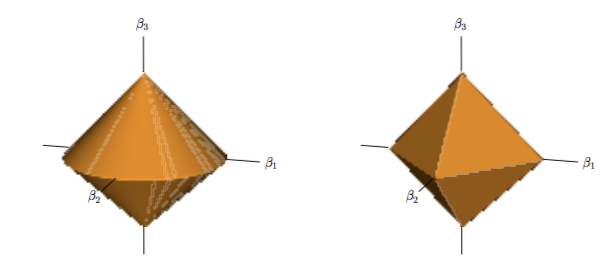
\includegraphics{fig/group_lasso.jpg}}
\caption{Til venstre ses kuglen for elastisk net med \(\alpha=0.7\) og til højre ses \(\ell_1\) kuglen for \(p=3\).}
\label{fig:elastisk_net}
\end{figure}
%
I \eqref{eq:4.5}, straffes alle grupper ligeligt, hvilket betyder at større grupper vil have en tendens til at blive valgt.
\citep{group_lasso} anbefalede at vægte strafleddene for hver gruppe i forhold til gruppens størrelse med en factor \(\sqrt{p_j}\).

\subsection{Udregning af group lasso}
\subsubsection{Coordinate descent}
Lad os omskrive optimeringsproblemet \eqref{eq:4.5} på matrix-vektor form
\begin{align*}
\argmin_{\theta_1, \ldots, \theta_J} \cbr{\frac{1}{2} \Vert \y - \sum_{j=1}^J \mathbf{Z}_{j} \theta_j \Vert_2^2 + \lambda \sum_{j=1}^J \Vert \theta_j \Vert_2}.
\end{align*}
For dette problem er nul subgradient ligningerne givet ved
\begin{align*}
- \mathbf{Z}_{j}^T \del{\y - \sum_{\ell=1}^J \mathbf{Z}_\ell \hat{\theta}_\ell} + \lambda \hat{s}_j = 0, \quad j=1,\ldots, J,
\end{align*} 
hvor $\hat{s}_j \in \R^{p_j}$ er et element af subdifferentialet af normen $\Vert \cdot \Vert_2$ evalueret i $\hat{\theta}_j$.
Når $\hat{\theta}_j \neq 0$ da har vi, at $\hat{s}_j = \frac{\hat{\theta}_j}{\Vert \hat{\theta}_j \vert_2}$, og når $\hat{\theta}_j=0$ da har vi, at $\hat{s}_j$ er enhver vektor hvor $\Vert \hat{s}_j \Vert_2 \leq 1$.
En metode at løse nul subgradent ligningerne er ved at fastholde alle block vektorer $\{\hat{\theta}_k, k \neq j\}$, og da løse for $\hat{\theta}_j$.
Hermed udføres block coordinate descent på objektfunktionen af group lasso.
Da problemet er konveks, og strafleddet kan separeres efter block, er det garanteret at konvergere til en optimal løsning.

Med $\{\hat{\theta}_k, k \neq j\}$ fastholdt, kan vi skrive
\begin{align*}
- \mathbf{Z}_{j}^T \del{\mathbf{r}_j - \mathbf{Z}_j \hat{\theta}_j} + \lambda \hat{s}_j = 0,
\end{align*}
hvor $\mathbf{r}_j = \y - \sum_{k \neq j} \mathbf{Z}_k \hat{\theta}_k $ er den j'te partial residual.
Fra betingelserne opfyldt af subgradienten $\hat{s}_j$, må vi have at $\hat{\theta}_j =0$ hvis $\Vert \mathbf{Z}_j^T \mathbf{r}_j \Vert_2 < \lambda$, og ellers må $\hat{\theta}_j$ opfylde
\begin{align}
\hat{\theta}_j = \del{\mathbf{Z}_j^T \mathbf{Z}_j + \frac{\lambda}{\Vert \hat{\theta}_j \Vert_2} \mathbf{I}}^{-1} \mathbf{Z}_j^T \mathbf{r}_j. \label{eq:4.14}
\end{align}
Denne opdatering er ens med løsningen af ridge regression, bortset fra at den underliggende strafparameter afhænger af $\Vert \hat{\theta}_j \Vert_2$.
Ligning \eqref{eq:4.14} har desværre ikke en lukket løsning for $\hat{\theta}_j$, medmindre at $\mathbf{Z}_j$ er ortonormal. I dette special tilfælde har vi, at
\begin{align*}
\hat{\theta}_j = \del{1 - \frac{\lambda}{\Vert \mathbf{Z}_j^T \mathbf{r}_j \Vert_2}}_+  \mathbf{Z}_j^T \mathbf{r}_j.
\end{align*}

\subsubsection{LARS}

\subsection{Sparse group lasso}
kompromis mellem group lasso og lasso
\newpage

\section{Ikke-negative garrote}
\textit{Ikke-negative garrote}, introduceret i \citep{nonnegative_garrote}, er en two-stage procedure. 
Givet et initial estimat af regression koefficienterne \(\tilde{\beta} \in \mathbb{R}^p\), kan vi løse optimeringsproblemet
\begin{align}
\hat{\beta}_j^\text{garotte} = \argmin_{c \in \mathbb{R}^p}  \cbr{ \sum_{i=1}^n \del{y_i - \sum_{j=1}^p c_j x_{ij} \tilde{\beta}_j}^2}, \ \text{underlagt at } c_j \geq 0 \text{ og } \Vert c \Vert_1 \leq t. \label{eq:2.19}
\end{align}
Lad \(\hat{\beta}_j^\text{garotte} = \hat{c}_j \cdot \tilde{\beta}_j\), for \(j = 1, \ldots, p\).
Der er et ækvivalent Lagrange problem for denne procedure
\begin{align}
\hat{\beta}_j^\text{garotte} = \argmin_{c \in \mathbb{R}^p}  \cbr{\Vert \y - \X \beta \Vert_2^2 + \lambda \Vert c \Vert_1}, \ \text{underlagt at } c_j \geq 0, \label{eq:nonnegative_garrote}
\end{align}
hvor \(\lambda \geq 0\).
Et tilstrækkelig høj \(\lambda\) shrinks nogle \(c_j\) til præcis nul.
I den originale artikel \citep{nonnegative_garrote}, er initial estimatet \(\tilde{\beta}\) valgt til at være \(\hat{\beta}_j^\text{OLS}\).

Antag \(\X\) er ortogonal og \(t\) er således at betingelsen \(\Vert c \Vert_1 = t\) er opfyldt, da er
\begin{align*}
\hat{c}_j = \del{1 - \frac{\lambda}{\tilde{\beta}_j^2}}_+, \ j = 1, \ldots, p,
\end{align*}
hvor \(\lambda\) er valgt således at \(\Vert \hat{c} \Vert_1 = t\).
Hvis koefficienten \(\tilde{\beta}_j\) er stor, da vil shrinkage faktoren være tæt på 1, dvs ingen shrinkage, men hvis den er lille, da vil estimatet blive shrunkage mod 0.
Af figur \ref{fig:nonnegative_garrote} ses det, at garrote shrinker lave værdier af \(\beta\) hårdere end lasso, og omvendt for høje værdier.
%
\begin{figure}[H]
\centering
\scalebox{0.8}{\begin{tikzpicture}
%\draw[loosely dotted] (-3,-3) -- (3,3);
%\draw[dotted] (-3,-2) -- (3,2);
%\draw (-3,-1.5) -- (-0.75,0) -- (0.75,0) -- (3,1.5);
\draw (-3,-3) -- (3,3);
\draw[dashed] (-3,-2.2) -- (-0.75,0) -- (0.75,0) -- (3,2.2);
\draw[dotted] (-3,-2.6) -- (-1,0) -- (1,0) -- (3,2.6);
\draw [<-] (0,3.5) node [left] {$\hat{\beta}$}-- (0,-3.5);
\draw[<-] (3.5,0) node [below] {$\beta$} -- (-3.5,0);
\end{tikzpicture}}
\caption[optional short text]{Eksakte løsninger for lasso (\tikz[baseline]{\draw[dashed] (0,.5ex)--++(.5,0) ;}) og nonnegative garrote (\tikz[baseline]{\draw[dotted] (0,.5ex)--++(.5,0) ;}).} \label{fig:nonnegative_garrote}
\end{figure}
%
Nonnegaitve garrote er tæt relateret med adaptive lasso, som vi vil diskutere nærmere i underafsnittet \ref{subsec:konsistentAL}.

-- viste at nonnegative garrote er path-konsistent under mindre strenge betingelser end lasso.
Dette gælder, hvis initial estimaterne er \(\sqrt{n}\)-konsistent, som inkluderer mindste kvadraters metoder (når \(p < n\)), lasso og elastisk net.
Path-konsistent betyder, at løsningsstien inkluderer den sande model.
Dog er konvergensen af parameter estimaterne for nonnegative garrote langsommere end den er for initial estimatet.


\section{Adaptive lasso}
Adaptive lasso blev introduceret i \citep{adaptive_lasso} og er endnu en udvidelse af standard lasso.
Ideen bag adaptive lasso er at tildele prædiktorernes koefficienter individuelle straffe, istedet for at alle koefficienter straffes ligeligt, som er tilfældet for standard lasso.
Den vægtede lasso er givet ved
\begin{align*}
\argmin_{\tbeta \in \R^p} \cbr{\Vert \y - \X \tbeta \Vert_2^2 + \lambda \sum_{j=1}^p w_j \vert \beta_j \vert},
\end{align*}
hvor \(\mathbf{w}\) er en kendt \(p \times 1\) vektor og \(w_j \geq 0\).

Adaptive lasso er blot en vægtet lasso, hvor vægtene \(\mathbf{w}\) er bestemt, således at metoden opfylder orakelegenskaberne, som vi vil bevise i afsnit \ref{subsec:konsistentAL}.
\begin{defn}[Adaptive lasso]
Antag \(\tilde{\tbeta}\) er rod-n konsistent til \(\tbeta^*\) (se definition \ref{def:rodn}).
Vælg \(\gamma>0\) og definer \(\widehat{\mathbf{w}} = \frac{1}{\vert \tilde{\tbeta} \vert^\gamma}\), da er adaptive lasso estimaterne givet ved
\begin{align}
\widehat{\tbeta}^\text{AL} = \argmin_{\tbeta \in \R^p} \cbr{ \Vert \y - \X \tbeta \Vert_2^2 + \lambda \sum_{j=1}^p \frac{ \vert \beta_j \vert}{\vert \tilde{\beta}_j \vert }^\gamma}. \label{eq:4.76}
\end{align}
\end{defn}
%Af sætning --- Der gælder, at \(\widehat{\tbeta}^\text{OLS}\) og \(\widehat{\tbeta}^\text{lasso}\) er rod-n konsistent.

\subsection{Udregning af adaptive lasso}
Givet \(\tilde{\tbeta}\) er optimeringsproblemet \eqref{eq:4.76} konveks, og kan dermed løses med coordinate descent og LARS algoritmen.
\subsubsection{Coordinate descent}
Opdateringerne for adaptive lasso i coordinate descent algoritmen er blot en simpel udvidelse af opdateringerne for standard lasso i afsnit \ref{subsec:udregning_lasso}.
For standardiserede prædiktorer og en centeret responsvariabel er coordinate descent opdateringen for $j$'te koefficient givet ved
\begin{align}
\widehat{\beta}^\text{AL}_j \del{\lambda}= S_{\frac{\widehat{\mathbf{w}} \lambda}{2n}} \del{\tilde{\beta}_j}, \label{eq:AL_coordinate_update}
\end{align}
hvor \(\tilde{\beta}_j = \frac{1}{n} \sum_{i=1}^n r_{i}^{(j)} x_{ij}\) og \(r_{i}^{(j)} = y_i - \sum_{k \neq j} x_{ik} \widehat{\beta}^\text{AL}_k \del{\lambda}\) er de partielle residualer.
Vi gennemløber opdateringen \eqref{eq:AL_coordinate_update} indtil konvergens.

\begin{eks}
På figur \ref{fig:diabetes_lasso_adaptivelasso} illustreres koefficientstierne for lasso og adaptive lasso med OLS vægte og \(\gamma = 1\) for diabetes data.
\imgfigh{diabetes_lasso_adaptivelasso.pdf}{0.9}{Koefficientstierne for lasso og adaptive lasso med OLS vægte og \(\gamma = 1\) som funktion af $\log \del{\lambda}$ for diabetes data.}{diabetes_lasso_adaptivelasso}

\end{eks}

\subsubsection{LARS}
Adaptive lasso problemet kan løses med LARS algoritmen ud fra følgende simple trin
\begin{enumerate}
\item Definér \(\mathbf{x}_j^{*} = \frac{\mathbf{x}_j}{\widehat{w}_j}\) for \(j=1, \ldots, p\)
\item Løs lasso problemet for alle \(\lambda_n\): \(\widehat{\tbeta}^{*} = \argmin_{\tbeta \in \R^p} \left\Vert \y - \sum_{j=1}^p \mathbf{x}_j^{*} \beta_j \right\Vert^2 + \lambda_n \sum_{j=1}^p \vert \beta_j \vert\)
%\begin{align*}
%\widehat{\tbeta}^{*} = \argmin_{\tbeta} \left\Vert \y - \sum_{j=1}^p \mathbf{x}_j^{*} \beta_j \right\Vert^2 + \lambda_n \sum_{j=1}^p \vert \beta_j \vert
%\end{align*}
\item Adaptive lasso estimatoren er da givet ved \(\widehat{\beta}_j^{\text{AL}} = \frac{\widehat{\beta}_j^{*}}{\widehat{w}_j}\)
\end{enumerate}
%computermæssige omkostninger er af orden \(O\del{np^2}\) svarende til et enkelt OLS fit.
%
%Antag vi anvendes \(\hat{\beta}^\text{OLS}\) til at konstruere vægtene i adaptive lasso, da ønsker vi at finde et optimal par af \(\del{\gamma, \lambda_n}\).
%For en given \(\gamma\), kan vi udføre to dimensionel krydsvalidering sammen med LARS algoritmen til at søge efter en optimal \(\lambda_n\).
%I princippet kan \(\hat{\beta}^\text{OLS}\) med andre rod-n konsistente estimatoren.
%Vi kan behandle den som en tredje tunning parameter og udføre en tre-dimensionel krydsvalidering til at finde en optimal triple \(\del{\hat{\beta}, \gamma, \lambda_n}\).
%I \citep{adaptive_lasso} foreslås \(\hat{\beta}^\text{OLS}\) medmindre kollinaritet er en bekymring, i dette tilfælde kan vi forsøge med \(\hat{\beta}^\text{ridge}\), da den er mere stabil end \(\hat{\beta}^\text{OLS}\).
%